\documentclass[12pt]{article}

\usepackage[T1]{fontenc}
\usepackage[utf8]{inputenc}
\usepackage[spanish]{babel}
\usepackage{graphicx}
\usepackage{amsmath}
\usepackage{amssymb, amsfonts, latexsym, cancel}
\usepackage{epstopdf}
\usepackage{float}
\usepackage{subfigure}
\usepackage{array}
\usepackage{longtable}
\usepackage{array}
%CAMBIAR CONFIGURACION DE ARRAY PARA USAR MAS DE 10 COLUMNAS
\setcounter{MaxMatrixCols}{40}
\usepackage{bm}
\parindent = 1cm

\newcolumntype{E}{>{$}c<{$}}

\begin{document}
\title{Utilizando \LaTeX}
\author{Maximiliano Ponce Marquez}
\date{2 de Octubre del 2019}
\maketitle

\newpage

\tableofcontents

\newpage

%\chapter{Texto}
\section{Tipos y tamaños de fuente}
Iniciamos con la segunda práctica de este tutorial,
colocando el título autor y día. Esta es la primera
sección donde conoceremos algunos tipos de letra, así
como los diferentes tamaños de letra que podemos usar
\subsection{Tipos de letra}
\begin{itemize}
\item Tipo de letra \textbf{negrita}
\item Tipo de letra \textit{itálica}
\item Tipo de letra \textrm{romana}
\item Tipo de letra \textsf{sans serif}
\item Tipo de letra \texttt{mono espaciada}
\item Tipo de letra \textsl{inclinada}
\item Tipo de letra \textsc{versalitas}
\end{itemize}

\newpage

\subsection{Tamaños de letra}
\begin{itemize}
\item {\tiny Tamaño de letra} tiny
\item {\scriptsize Tamaño de letra} scriptsize
\item {\footnotesize Tamaño de letra} footnotesize
\item {\small Tamaño de letra} small
\item {\normalsize Tamaño de letra} normalsize
\item {\large Tamaño de letra} large
\item {\Large Tamaño de letra} Large
\item {\LARGE Tamaño de letra} LARGE
\item {\huge Tamaño de letra} huge
%\item {\HUGE Tamaño de letra} HUGE
\end{itemize}

\section{Párrafos, sangría y saltos de línea}
\subsection{Sangría}
Iniciamos con la segunda práctica de este tutorial,
colocando el título autor y día. Esta es la primera
sección donde conoceremos algunos tipos de letra, así
como los diferentes tamaños de letra que podemos usar
Texto de ejemplo aqui \textbf{si hay sangría} 

\noindent Iniciamos con la segunda práctica de este tutorial,
colocando el título autor y día. Esta es la primera
sección donde conoceremos algunos tipos de letra, así
como los diferentes tamaños de letra que podemos usar
Texto de ejemplo aqui \textbf{no hay sangría} 

\newpage

\subsection{Salto de línea y nueva página}
Ahora queremos también decidir y modificar la sangría en el
documento, aquí iniciamos con sangría. \\
Esta es otra línea \par
Esta es otra línea pero con sangría \\[0.5cm]
Otra línea con un espacio más grande

\subsection{Alineación de párrafos}
\begin{flushleft}
Texto a la izquierda
\end{flushleft}
\begin{center}
Texto centrado
\end{center}
\begin{flushright}
Texto a la derecha
\end{flushright}

\subsection{Comillas y puntos suspensivos}
Este es un ejemplo: ``para comillas simples'', `simples' y ``dobles'' \\
Y también los puntos suspensivos \dots

\subsection{Espaciado horizonal}
\noindent Inicio \, fin\\[0.2cm]
\noindent Inicio \quad fin\\[0.2cm]
\noindent Inicio \qquad fin\\[0.2cm]
\noindent Inicio \hspace{3cm} fin\\[0.2cm]
\noindent Inicio \hfill fin\\[0.2cm]

\subsection{Líneas de relleno}
\noindent Inicio \, fin\\[0.5cm]
Inicio \hrulefill fin\\[0.2cm]
Inicio \dotfill fin\\[0.2cm]

%\chapter{Modo matemático}

\section{Ecuaciones en línea e independientes}

\subsection{Ecuación en línea}
\textbf{Cuadrado de un binomio} Sea $(a+b)^2$ donde $a$ y $b$ representan variables algebraicas. Por lo tanto $(a+b)^2=a^{2}+2ab+b{2}$

\subsection{Ecuación independiente}
\textbf{Cuadrado de un binomio} Sea $(a+b)^2$ donde $a$ y $b$ representan variables algebraicas. Por lo tanto 
\[ (a+b)^2=a^{2}+2ab+b^{2} \]
\begin{equation*}
	(a+b)^2=a^{2}+2ab+b^{2}
\end{equation*}
\subsection{Numeración de fórmulas y referencia}
Ecuaciones con número
\begin{equation}\label{binomio1}
	(a+b)^2=a^{2}+2ab+b^{2}
\end{equation}
\begin{equation}\label{binomio2}
	(x+y)^2=x^{2}+2xy+y^{2}
\end{equation}
Ahora usando la ecuación 1 por referencia \ref{binomio1} y ecuación 2 por referencia \ref{binomio2} \\
Ahora usando la ecuación 1 por referencia \eqref{binomio1} y ecuación 2 por referencia \eqref{binomio2}

\subsection{Alinear ecuaciones con el comando alinq}
\begin{align}
x &= a = b\\
y &= 2a + b\\
z &= 3a + 2b
\end{align}
Sin referencia
\begin{align*}
x &= a = b\\
y &= 2a + b\\
z &= 3a + 2b
\end{align*}

\begin{align}
x &= a = b   & x &= a = b   & x &= a = b\\
y &= 2a + b  & y &= 2a + b  & y &= 2a + b\\
z &= 3a + 2b & z &= 3a + 2b & z &= 3a + 2b
\end{align}

\begin{align}
x &= a = b\\
y &= 2a + b\nonumber \\
z &= 3a + 2b \nonumber 
\end{align}
\begin{align}
x &= a = b\\
  &= 2a + b\nonumber \\
  &= 3a + 2b \nonumber 
\end{align}

\subsection{Fracciones}
\begin{itemize}
\item Junto a texto $ \frac{x}{y}$
\item Junto a texto $ \dfrac{x}{y}$
\item Junto a texto \[\frac{x}{y}\]
\end{itemize}

\subsection{Potencias, subíndices y superíndices}
\begin{itemize}
\item Potencia $ x^{6}$
\item Subíndice $z_{3}$
\item Superíndice \[a^{x^{2}}\]
\end{itemize}

\subsection{Raíces}
\begin{itemize}
\item Raíz cuadrada $ \sqrt{a+b}$
\item Raíz n-ésima $ \sqrt[n]{a+b}$
\item \[\sqrt[n]{a+b}\]
\end{itemize}

\subsection{Coeficientes binomiales}
\begin{itemize}
\item Junto a texto $ \binom{n}{k}$
\item \[\binom{n}{k}\]
\end{itemize}

\section{Gráficas}

\subsection{Incluir gráficas externas}
En \LaTeX podemos incluir gráficas externas o generadas
directamente en \LaTeX , utilizando algún paquete, algunos de los formatos que podemos utilizar son \textbf{.jpg}, \textbf{.png}, \textbf{.eps} y \textbf{pdf}.\\[0.5cm]
Los formatos vectoriales como lo son \textbf{.eps} y \textbf{.pdf} son los mas recomendados cuando hacemos gráficas en las cuales queremos observar detalles y precisión, porque no pierden calidad al aumentar o disminuir su tamaño. y para imágenes en general podemos utilizar los formatos \textbf{.jpg} o \textbf{.png}

\subsection{Paquete graphicx}
\begin{center}

\includegraphics[scale=0.4]{figuras/imagen1.pdf}
\end{center}
\begin{itemize}
\item scale: Escala la imagen.
\item width: Ancho deseado de la imagen en cm.
\item height: Altura deseada de la imagen en cm.
\end{itemize}

\begin{center}

\includegraphics[scale=0.1]{figuras/imagen1.pdf} \quad

\includegraphics[scale=0.2]{figuras/imagen1.pdf} \quad

\includegraphics[scale=0.3]{figuras/imagen1.pdf} \quad

\includegraphics[scale=0.4]{figuras/imagen1.pdf} \quad
\end{center}

\begin{center}

\includegraphics[width=4cm]{figuras/imagen1.pdf}
\end{center}

\begin{center}

\includegraphics[height=5cm]{figuras/imagen1.pdf}
\end{center}

\newpage
\subsection{Objetos flotantes}
En \LaTeX podemos incluir gráficas externas o generadas
directamente en \LaTeX , utilizando algún paquete, algunos de los formatos que podemos utilizar son \textbf{.jpg}, \textbf{.png}, \textbf{.eps} y \textbf{pdf}.\\[0.5cm]

\begin{figure}[!ht]
\centering
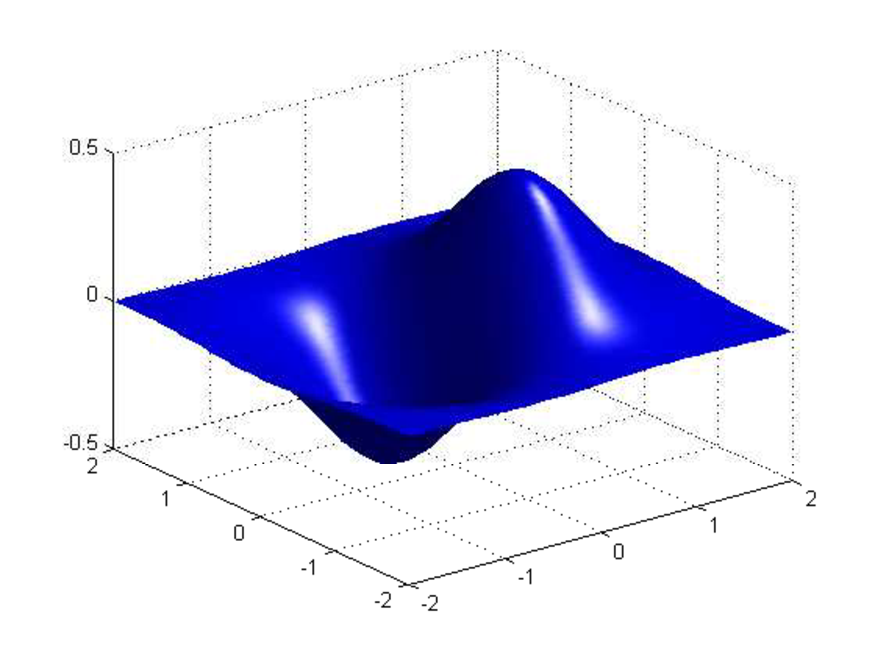
\includegraphics[scale=0.5]{figuras/imagenmat.pdf} 
\put(-100,50){\footnotesize{usando el comando put}}
\put(0,0){$x+1$}
\caption{Imagen a escala 0.5}
\label{Figura 1}
\end{figure}

Los formatos vectoriales como lo son \textbf{.eps} y \textbf{.pdf} son los mas recomendados cuando hacemos gráficas en las cuales queremos observar detalles y precisión, porque no pierden calidad al aumentar o disminuir su tamaño. y para imágenes en general podemos utilizar los formatos \textbf{.jpg} o \textbf{.png}

\begin{itemize}
\item t: La imagen en la parte superior (top)
\item b: La imagen en la parte inferior (bot)
\item h: La imagen en el sitio que escribimos (here)
\item H: del paquete float, permite colocar la imagen donde debe estar, sin brincar a otra página
\end{itemize}

\begin{figure}[H]
\centering
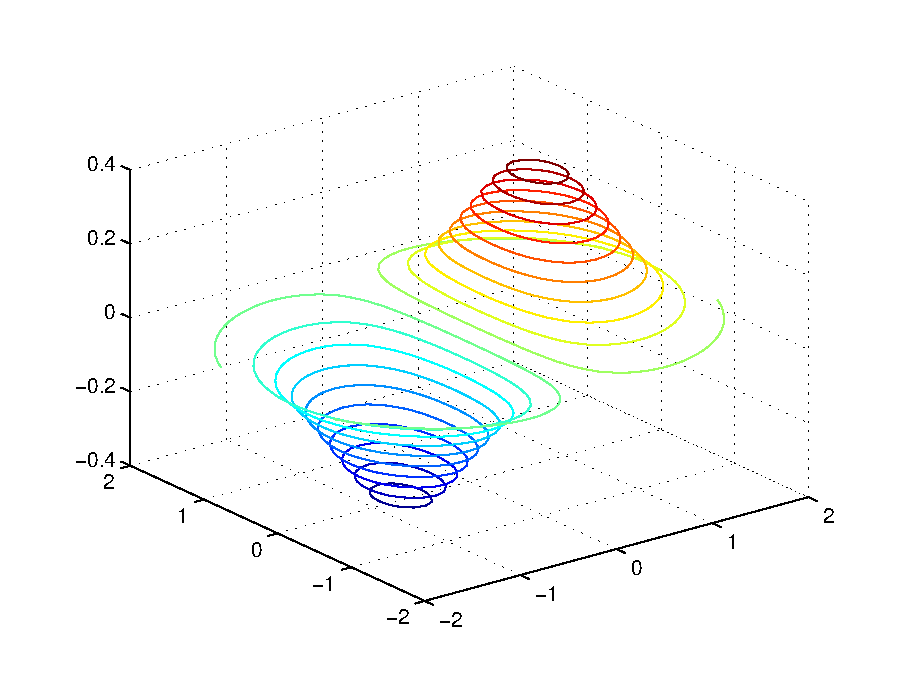
\includegraphics[scale=0.5]{figuras/imagenmat2.eps} 
\caption{Imagen eps}
\label{Figura 1}
\end{figure}

\newpage
\subsection{Paquete float}

\begin{figure}[H]
\centering
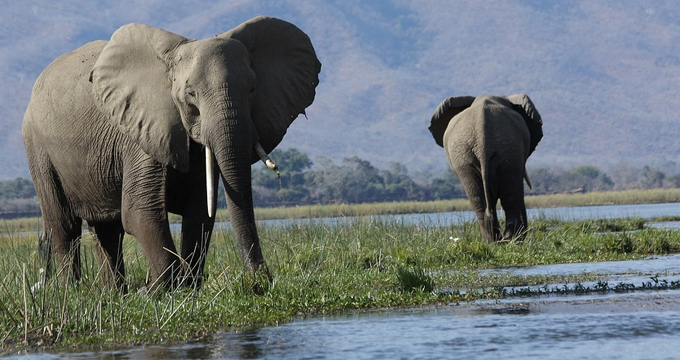
\includegraphics[scale=0.3]{figuras/elefante} 
\caption{Imagen con formata jpg}
\label{figura2}
\end{figure}

Como lo muestra la imgaen \eqref{figura2}
En \LaTeX podemos incluir gráficas externas o generadas
directamente en \LaTeX , utilizando algún paquete, algunos de los formatos que podemos utilizar son \textbf{.jpg}, \textbf{.png}, \textbf{.eps} y \textbf{pdf}.\\[0.5cm]
Los formatos vectoriales como lo son \textbf{.eps} y \textbf{.pdf} son los mas recomendados cuando hacemos gráficas en las cuales queremos observar detalles y precisión, porque no pierden calidad al aumentar o disminuir su tamaño. y para imágenes en general podemos utilizar los formatos \textbf{.jpg} o \textbf{.png}

\begin{figure}[H]
\centering
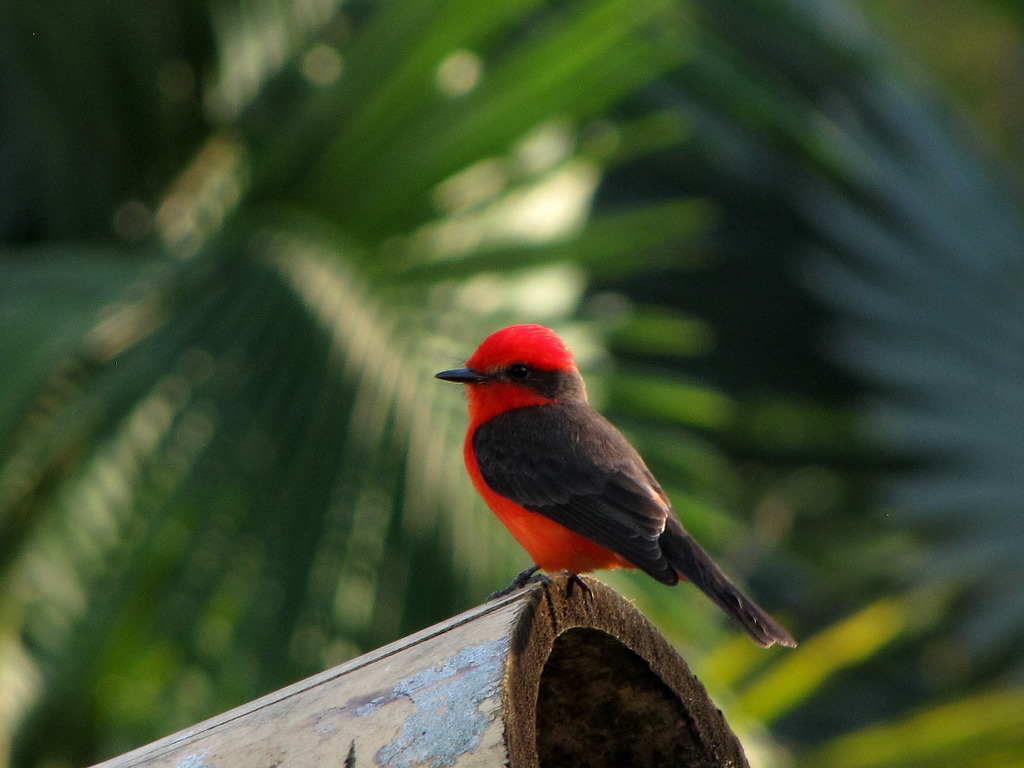
\includegraphics[scale=0.15]{figuras/Petirrojo2} 
\caption{Imagen con formata jpg}
\label{figura3}
\end{figure}

\newpage
\subsection{Paquete subfigure}
\begin{figure}[!ht]
\centering

\subfigure[Primera figura]
{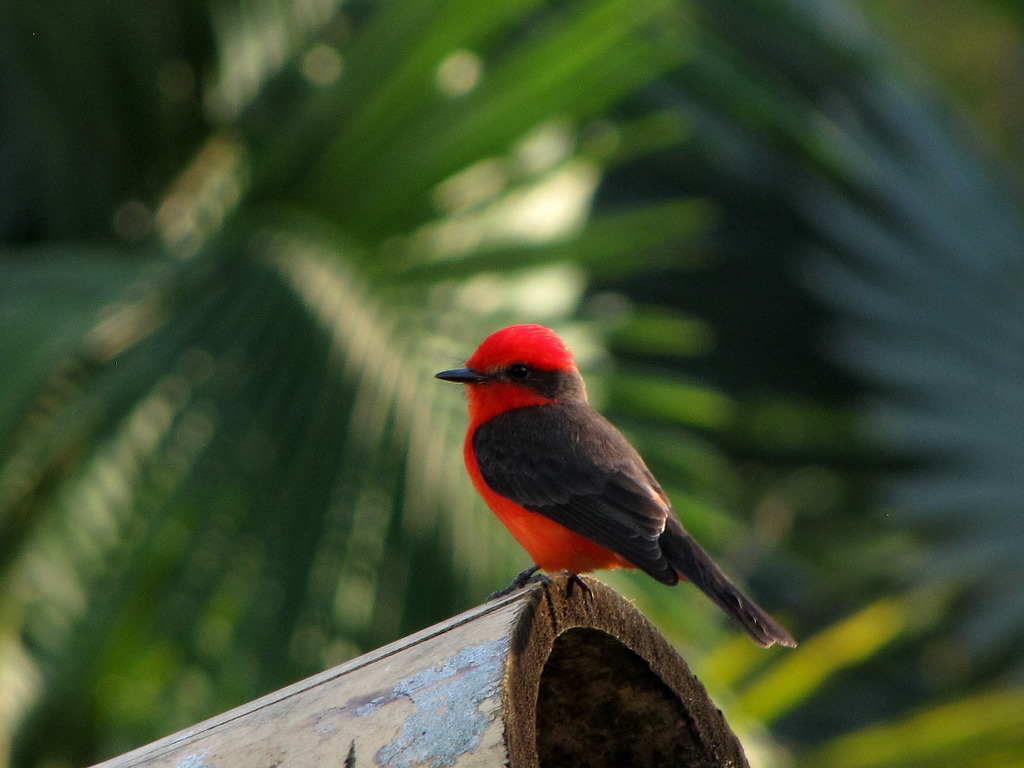
\includegraphics[scale=0.1]{figuras/Petirrojo2} }
\quad
\subfigure[Segunda figura]
{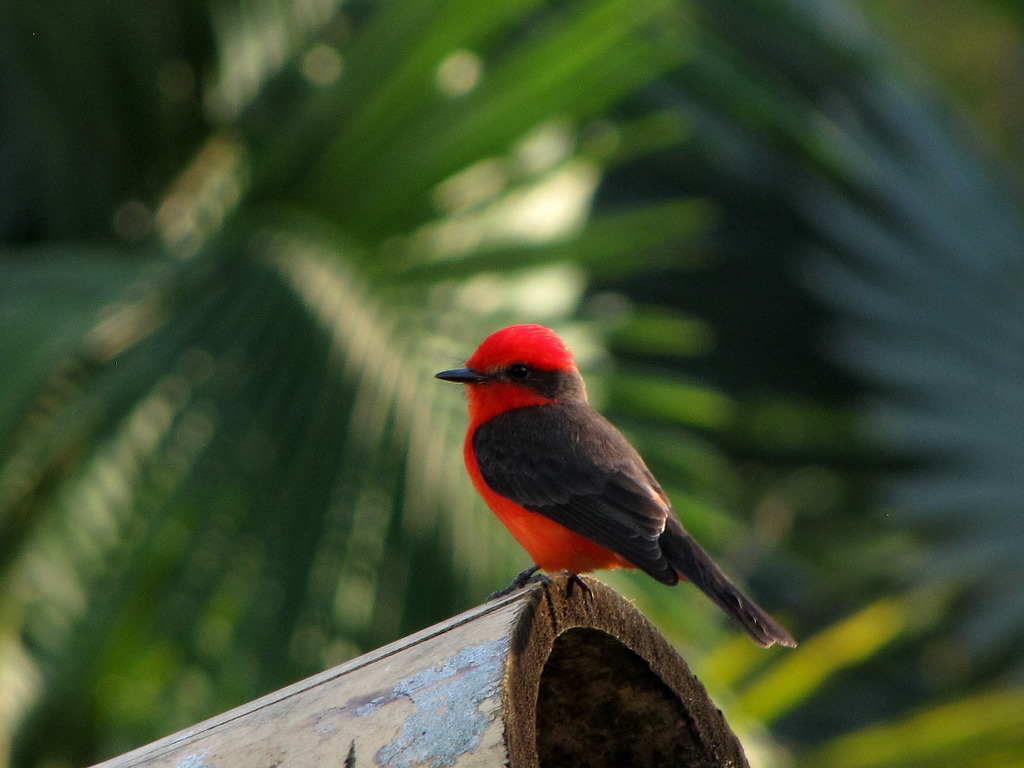
\includegraphics[scale=0.1]{figuras/Petirrojo2} }
\quad
\subfigure[Tercera figura]
{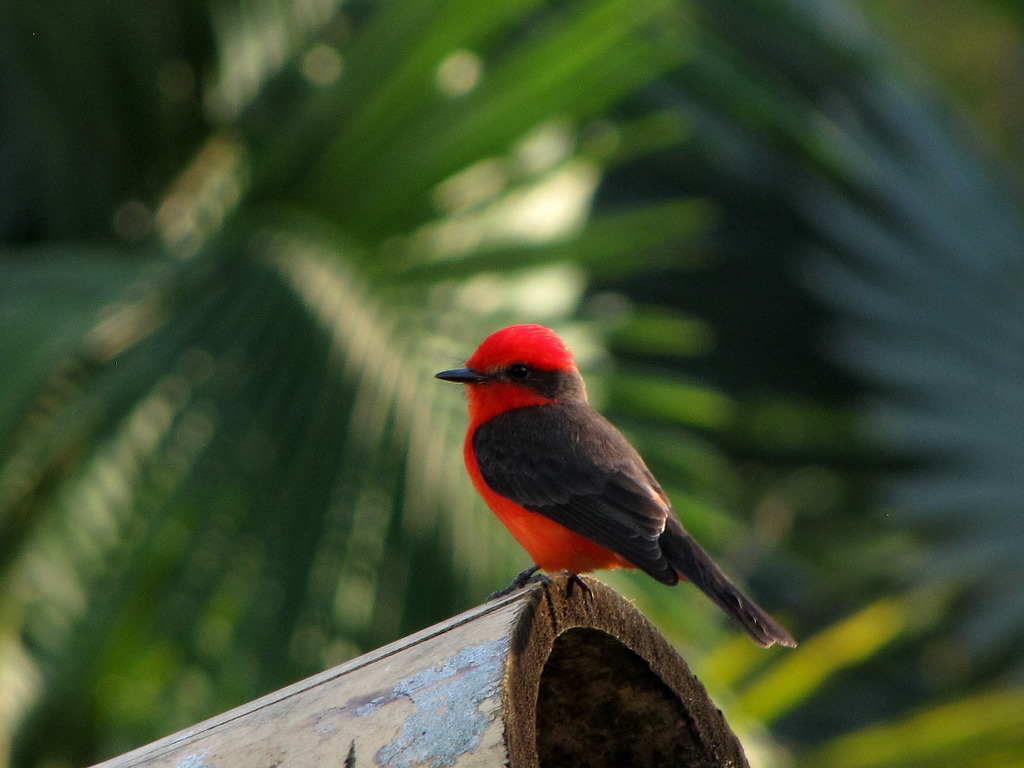
\includegraphics[scale=0.1]{figuras/Petirrojo2} }
\caption{Imagen con formata jpg}
\label{figuraVarias}
\end{figure}

Tal como aparece en la figura anterior \eqref{figuraVarias}

\section{Tablas básicas}
En \LaTeX \, la forma básica en la que podemos incluir tablas es usanto el entorno \textbf{tabular}, su síntaxis es la siguiente.\\[0.3cm]
\noindent \textbf{Formato de las columnas:}
\begin{itemize}
\item l (alineado a la izquerda)
\item c (alineación centrada)
\item r (alineado a la derecha)
\end{itemize}
\begin{itemize}
\item $\&$ Cáracter que se utiliza para separar columnas
\end{itemize}
	
Nuestra primera tabla \quad
\begin{table}[!ht]
\centering
\begin{tabular}{ccc}
\hline
Lunes & Martes & Miercoles \\
\hline
0 & 0 & 0 \\
\hline
1 & 1 & 1 \\
\hline
\end{tabular}
\caption{tabla con líneas}
\label{incluirimagen}
\end{table}

\begin{table}[!ht]
\centering
\begin{tabular}{|l|c|r|c|}
\hline
Lunes & Martes & Miercoles & Jueves\\
\cline{1-2}
0 & 0 & 0 & 0 \\
\cline{1-3}
1 & 1 & 1 & 1 \\
\hline
\end{tabular}
\caption{tabla con líneas de diferente tamaño}
\label{lineas}
\end{table}
\newpage
Ejemplo de tablas con líneas de diferente tamaño

\begin{table}[H]
\centering
\begin{tabular}{|l|c|r|c|}
\hline
Lunes & Martes & Miercoles & Jueves\\
\cline{2-4}
0 & 0 & 0 & 0 \\
\cline{3-4}
1 & 1 & 1 & 1 \\
\hline
\end{tabular}
\caption{tabla con líneas de diferente tamaño}
\label{lineas}
\end{table}

\subsection{Multiples columnas}
\begin{table}[H]
\centering
\begin{tabular}{|l|c|r|c|}
\hline
\multicolumn{2}{|c|}{Enero} & & \\
\hline
\multicolumn{4}{|c|}{Días de la semana} \\
\hline
& \multicolumn{3}{|c|}{Días de la semana} \\
\hline
Lunes & Martes & Miercoles & Jueves\\
\cline{2-4}
0 & 0 & 0 & 0 \\
\cline{3-4}
1 & 1 & 1 & 1 \\
\hline
\end{tabular}
\caption{tabla con líneas de diferente tamaño}
\label{lineas}
\end{table}

\subsection{Tablas con párrafos}
\begin{table}[H]
\centering
\begin{tabular}{|l|p{6cm}|}
\hline
Comando & Descripción \\
\hline
p$\{$Ancho$\}$ & Crea una sola columna con un ancho fijo. En el contenido de esta celda se compone de un párrafo ordinario, sin sangría inicial\\
\hline
m$\{$Ancho$\}$ & Crea una sola columna con un ancho fijo. El párrafo aparece verticalmente centrado respecto a las columnas vecinas\\
\hline
\end{tabular}
\caption{tabla con párrafos}
\label{lineas}
\end{table}
\begin{table}[H]
\centering
\begin{tabular}{|l|m{6cm}|}
\hline
Comando & Descripción \\
\hline
p$\{$Ancho$\}$ & Crea una sola columna con un ancho fijo. En el contenido de esta celda se compone de un párrafo ordinario, sin sangría inicial\\
\hline
m$\{$Ancho$\}$ & Crea una sola columna con un ancho fijo. El párrafo aparece verticalmente centrado respecto a las columnas vecinas\\
\hline
\end{tabular}
\caption{tabla con párrafos}
\label{lineas}
\end{table}

\subsection{Escalar una tabla}
\begin{table}[H]
\centering
\scalebox{0.7}{
\begin{tabular}{|l|m{6cm}|}
\hline
Comando & Descripción \\
\hline
p$\{$Ancho$\}$ & Crea una sola columna con un ancho fijo. En el contenido de esta celda se compone de un párrafo ordinario, sin sangría inicial\\
\hline
m$\{$Ancho$\}$ & Crea una sola columna con un ancho fijo. El párrafo aparece verticalmente centrado respecto a las columnas vecinas\\
\hline
\end{tabular}}
\caption{tabla escalada}
\label{lineas}
\end{table}
\newpage
\subsection{Expresiones matemáticas en tablas}
Tablas con expresiones

\begin{table}[H]
\centering	
\begin{tabular}{|l|c|c|}
\hline
matemática & $x+1$ & $\lambda$ \\
\hline
ejemplo & $x_{2}$ & $x_{3}$\\
\hline
$(a+b)^{2}$ & $(a+b)^{3}$ & $(a+b)^{4}$\\
\hline
\end{tabular}
\caption{Expresiones matemáticas de forma manual}
\end{table}

\begin{table}[H]
\centering	
\begin{tabular}{|E|E|E|}
\hline
x & x+1 & \lambda \\
\hline
x_1 & x_{2} & x_{3}\\
\hline
(a+b)^{2} & (a+b)^{3} & (a+b)^{4}\\
\hline
\end{tabular}
\caption{Expresiones matemáticas de forma automático}
\end{table}

\subsection{Tablas largas, paquete longtable}
\begin{longtable}[c]{|ccc|}
Nombre & Teléfono & Edad \\
Nombre & Teléfono & Edad \\
Nombre & Teléfono & Edad \\
Nombre & Teléfono & Edad \\
Nombre & Teléfono & Edad \\
Nombre & Teléfono & Edad \\
Nombre & Teléfono & Edad \\
Nombre & Teléfono & Edad \\
Nombre & Teléfono & Edad \\
A & 12345 & 20 \\
Nombre & Teléfono & Edad \\
Nombre & Teléfono & Edad \\
Nombre & Teléfono & Edad \\
Nombre & Teléfono & Edad \\
Nombre & Teléfono & Edad \\
Nombre & Teléfono & Edad \\
Nombre & Teléfono & Edad \\
Nombre & Teléfono & Edad \\
Nombre & Teléfono & Edad \\
A & 12345 & 20 \\
Nombre & Teléfono & Edad \\
Nombre & Teléfono & Edad \\
Nombre & Teléfono & Edad \\
Nombre & Teléfono & Edad \\
Nombre & Teléfono & Edad \\
Nombre & Teléfono & Edad \\
Nombre & Teléfono & Edad \\
Nombre & Teléfono & Edad \\
Nombre & Teléfono & Edad \\
A & 12345 & 20 \\
Nombre & Teléfono & Edad \\
Nombre & Teléfono & Edad \\
Nombre & Teléfono & Edad \\
Nombre & Teléfono & Edad \\
Nombre & Teléfono & Edad \\
Nombre & Teléfono & Edad \\
Nombre & Teléfono & Edad \\
Nombre & Teléfono & Edad \\
Nombre & Teléfono & Edad \\
A & 12345 & 20 \\
\caption{Tabla larga}
\label{TablaLargaEjemplo}
\end{longtable}

\section{Símbolos de agrupación}
\[ 
w + ( \frac{d}{b+c} )  = (a+b+c)
\]
\[ 
w + \left( \frac{d}{b+c} \right)  = (a+b+c)
\]
\[ 
w + \left\lbrace  \frac{d}{b+c} \right\rbrace   = (a+b+c)
\]

\[ 
\left\lbrace 
\frac{a+b}{c+d}
\right. 
\]

\begin{equation}
\left( 
\frac{a+b}{c+d}
\right\rbrace 
\end{equation}

\begin{equation}
\left( 
\frac{a+b}{c+d}
\right) ^{2}
\end{equation}

\begin{equation}
\left.
\frac{dy}{dx}
\right|_{x=1}=x+1
\end{equation}

\subsection{Tamaño manual}
\[
(\sum_{i=1}^n)
\]

\[
\bigl(
\sum_{i=1}^n
\bigr)
\]

\[
\Bigl(
\sum_{i=1}^n
\Bigr)
\]

\[
\biggl(
\sum_{i=1}^n
\biggr)
\]

\[
\Biggl(
\sum_{i=1}^n
\Biggr)
\]

\section{Matrices}
\subsection{Matrices usando el entorno Array}

\[
\begin{array}{lc}
0 & 1 \\
2 & 3
\end{array}
\]

\[
\left[ 
\begin{array}{lc}
0 & 1 \\
2 & 3
\end{array}
\right] 
\]

\[
\left[ 
\begin{array}{lrl}
0 & x & 1 \\
1 & x+1 & 2 \\ 
10 & x+y+1 & 3
\end{array}
\right] 
\]

\newpage

\subsection{Matrices con entornos predefinidos}
\[
\begin{matrix}
0 & 1 & 2 \\
0 & 1 & 2 \\
0 & 1 & 2 \\
\end{matrix}
\]

\[
\begin{pmatrix}
0 & 1 & 2 \\
0 & 1 & 2 \\
0 & 1 & 2 \\
\end{pmatrix}
\]

\[
\begin{bmatrix}
0 & 1 & 2 \\
0 & 1 & 2 \\
0 & 1 & 2 \\
\end{bmatrix}
\]

\[
\begin{vmatrix}
0 & 1 & 2 \\
0 & 1 & 2 \\
0 & 1 & 2 \\
\end{vmatrix}
\]

\[
\begin{Bmatrix}
0 & 1 & 2 \\
0 & 1 & 2 \\
0 & 1 & 2 \\
\end{Bmatrix}
\]
\\
\[
\begin{Vmatrix}
0 & 1 & 2 \\
0 & 1 & 2 \\
0 & 1 & 2 \\
\end{Vmatrix}
\]

\subsection{Máximo número de columnas}
\[
\begin{bmatrix}
0 & 1 & 2 & 3 & 4 & 5 & 6 & 7 & 8 & 9 \\
0 & 1 & 2 & 3 & 4 & 5 & 6 & 7 & 8 & 9 \\
\end{bmatrix}
\]

\[
\begin{bmatrix}
0 & 1 & 2 & 3 & 4 & 5 & 6 & 7 & 8 & 9 & 10 & 11 & 12 & 13\\
0 & 1 & 2 & 3 & 4 & 5 & 6 & 7 & 8 & 9 & 10 & 11 & 12 & 13\\
\end{bmatrix}
\]

\section{Negritas}

\textbf{Esto} esta en negritas $ \boldsymbol{a+b} $
\[
a+b
\]
\[
\boldsymbol{
a+b}
\]
\[
\bm{a+b}
\]


\begin{table}{H}
\begin{tabular}{E|E|E}
\text{Texto normal} & \text{Usando boldsymbol} & \text{Usando bm} \\
x+1 & \boldsymbol{x+1} & \bm{x+1}\\
x^{2} & \boldsymbol{x^{2}} & \bm{x^{2}}\\
\sum x+2 & \boldsymbol{\sum x+2} & \bm{\sum x+2}\\
\tan x & \boldsymbol{\tan x} & \bm{\tan x}\\
\end{tabular}
\end{table}


\end{document}




